\chapter{Event Evolution and Tracking}
A lot of research is going on to study the evolution of events over time in general. \cite{yang2014finding} studied common patterns and progression stages in event sequences like medical records, reviews of products and services and web/search logs. They build a generative model to study the common patterns in general event evolution. They assigned different classes to different sequences on the basis of their evolution hierarchy. \cite{duygulu2004towards} in their work tracked evolution of news stories for the purpose of event summarization. The core idea of their work is based on visual cues and textual information. News channels often repeat shots of a video multiple times during news broadcast. They have exploited this observation and used visual cues to detect repeating videos in a news to keep track of an event evolving over time. Evolution of events within a topic related to an incident using online news has been studied by \cite{yang2009discovering}. Significant research efforts have been made to study evolution of events in general. However, the effects of LDA-segmented tweets-cum-events on their tracking and evolution has not been studied in the past.

We didn't delved into complex methods of event tracking and evolution since our pipeline has already has identified event's major keywords. We represented each event as a cluster of topical words and use the well known Maximum Weighted Bipartite Matching algorithm for evolution and tracking.

\section{Problem Formulation}

A particular day’s event clusters obtained at the previous stage of the pipeline are grouped together to form one side of the bipartite graph same as in the bipartite graph matching problem. Now edges are constructed between event clusters of consecutive day’s events based on the similarity between the event clusters. Thus, forming an event chain over time showing the evolution and also it’s relation with other event chains on the social media.

The similarity between two event clusters on consecutive days is determined by the ratio obtained from adding the multiplied tweet frequency of the common topical words in the two event clusters and then dividing by the number obtained in the numerator plus the sum of the tweet frequency of the uncommon topical words in the two event clusters. The ratio obtained for the two event clusters determines the weight of the edge between them if above a certain threshold. On the other hand, if the ratio is below a certain threshold then no edge is constructed between the two events. Formally $s$ is the similarity between two clusters and its is defined as ratio of sum of frequency of intersection word set $I$ to the sum of frequency of union word set $U$.
\begin{equation}
s = \frac{\sum_i f_i \in I}{\sum_j f_j \in U}
\end{equation}
In this way, it is assured that event chain is constructed for related events only and thus is showing the actual progress of the event over time on social media. This whole process can be easily understood from the diagram given below.

\begin{figure*} 
    \centering 
    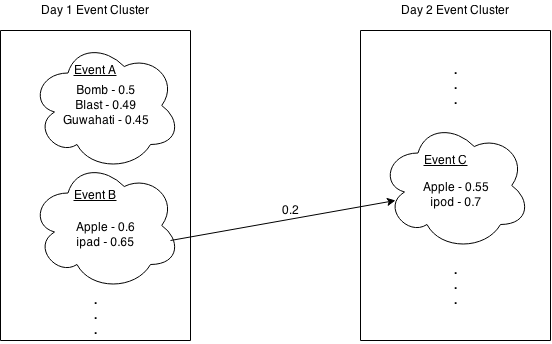
\includegraphics[width=0.9\textwidth]{Evolution1.png} 
    \caption{Formulation of event tracking as bipartite graph} 
    \label{fig:eventtracking}
\end{figure*}

We can see from the diagram that there is no edge between event A and event C because of the low similarity ratio between them as should be the actual case. Since, there is no connection between a “Bomb Blast” and an event related to “Apple Inc.”. Whereas, there is an event edge between event B and event C as should be the actual case. Since, it shows the product release activity of “Apple Inc.” which is relevant. So, we can say that our approach for constructing an event chain is in line with the actual event chains that exists in the social media.